\section{EASIER}
EASIER is a radio detector concept, it is composed of a radio sensor and an adaptation electronics embedded in the surface detector of the Pierre Auger Observatory, its main component are sketched on the Fig.~\ref{fig:diagram}. This concept was implemented in three bandwidths: the VHF band (30-80 MHz), the L band (1-1.5GHz) and the C-band (3.4-4.2GHz). We focus in this article only on the C-band. The  EASIER experiment  is one  of the  three C-band experiments  deployed at  the  Pierre Auger  Observatory site  besides AMBER~\cite{Gorham} and MIDAS~\cite{midas}. All of these setups intend to observe the molecular Bremsstrahlung radiation emitted from the ionization electrons of the shower. Contrary to AMBER and MIDAS which instrument an array of feed  horn antennas illuminated by a parabolic  dish, EASIER  relies on the observation of the shower  from the  ground with  a wide  angle antenna  pointing up in the sky.
A first array of 61 antennas called EASIER61 is running  since  2011 and has reported the observation of radio signals from EAS but at small distances from the shower axis. New estimations of the expected intensity led us to implement a new array, called GIGADuck, with an enhanced sensitivity installed since March 2015. These arrays are presented in this section.  
\subsection {The noise environment in the Pierre Auger Observatory site}
Radio measurement are often hindered by man made noise. Prior to  the installation,  we made sure that the environment at the Pierre Auger Observatory was radio quiet in the C-band.  The Fig.~\ref{fig:Pampa_spec} shows the noise spectrum measured  with  a C-band  LNBf  in the  Pampa Amarilla. The gain of the amplifier used is roughly \unit[60]{dB}, the background noise is thus around \unit[-180]{dBm/Hz} in the band. No strong peak is observed above this level in the tens of spectra recorded.
 \begin{figure}[!h]
  \center {
  \subfigure{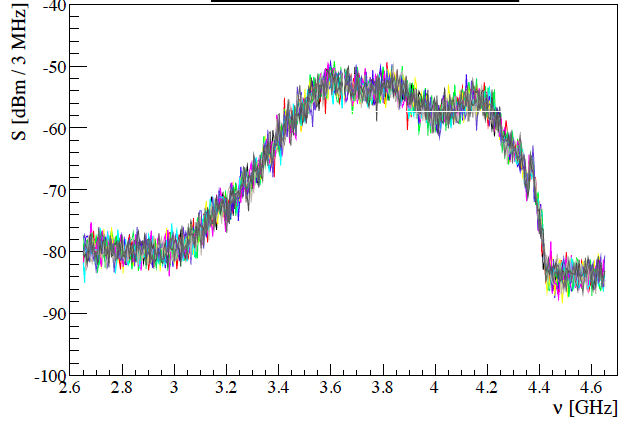
\includegraphics[width=0.49\linewidth]{Pampa_spec}}
    \subfigure{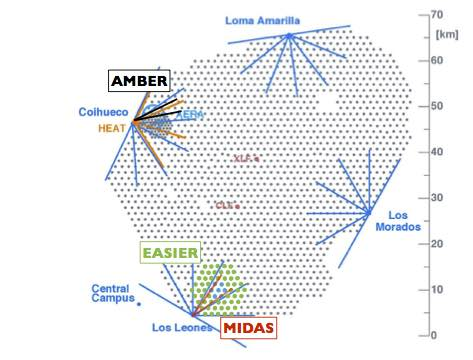
\includegraphics[width=0.49\linewidth]{augerarray.jpg}}  
  \caption{\small{Left:Frequency spectra in the C-band recorded in Pampa Amarilla. (The amplifier gain is around 60dB). Right: Footprint of EASIER array phase 1 (blue dots) and phase 2 (green dots).}}
  \label{fig:Pampa_spec}
    } 
\end{figure}

\subsection{The experimental setup}  
The basis of the EASIER detector is the  Pierre Auger  Observatory surface  detector. The Pierre Auger SD is  composed  of 1660 local stations arranged  in a tringular grid of  1500m spacement (see Fig.~\ref{fig:Pampa_spec}). Each local station is a water  Cherenkov detector equipped with three PMTs, a       local        acquisition       and       a       communication system, see~\cite{augerdetector} for a comprehensive description. An EASIER detector unit is designed to be integrated  into the  SD station.
 The receiver is a commercial horn antenna (Fig.~\ref{fig:detector}) made
 of a  feed and a  quarter wave length  monopole at its bottom.   It is
 tuned  for  a  central  frequency  of  3.8  GHz  and  a  bandwidth  of
 approximately \unit[500 to 800]{MHz}.  It  is associated with a low  noise block (LNB)  which amplifies  the signal by approximately  \unit[60]{dB} and lowers
 down the  central frequency to  \unit[1.35]{GHz}. The antenna and the LNB will be refered to LNBf within this document. A bias  tee is  inserted to provide  the power  supply to the  LNB and operate   the   transmission   of   the   RF  signal   on   a   single \unit[75]{$\Omega$} line.  Depending on  the setup, the line impedance  is adapted to \unit[50]{$\Omega$} by a resistor bridge.
 %% inducing a loss of  \unit[5.7]{dB}. 
 Potential low  frequency noises are filtered out  by a \unit[900]{MHz}
 high pass filter.  A logarithmic amplifier (minicircuit AD8318) serves
 as  a power  detector and outputs  a voltage  proportional to  the
 logarithm of the RF input power.   This model was chosen for its large
 frequency  bandwidth and  a fast  time response  of $\simeq$\unit[tens
   of]{ns} nominally.  This voltage is  in turn adapted to fit into  the local station  front  end, originally built to accept  PMT's negative voltage between 0 and
  -2V.  The EASIER  final analogic signal replaces one  of the low gain
  channel of  the local station (each local  station acquires ordinarly
  the last  dynode and the  anode of three  PMTs, the anode  being used
  only  in  case of  saturation  of the  dynode).   The  final part  of
  acquisition includes an antialiasing filter cutting frequencies above
  \unit[20]{MHz} and the FADC digitizer sampling a \unit[19.2]{$\mu$ s}
  waveform at a  \unit[40]{MHz} rate and coding the  analogic signal on
  10 bits~\cite{augertechnical}.   The data stream is then  sent to the
  central acquisition and the  reconstruction of the event is performed
  independently of the radio signal. As a consequence, no separated trigger for the radio signal is needed and the EASIER data are simply part of the regular SD data stream.  As  an additional benefit, the radio detector
is  powered by the  station battery  and is  also integrated  into the SD station's monitoring  system. 

\begin{figure}[!ht]
  \centering
  \hspace*{-3ex}  
  \subfigure{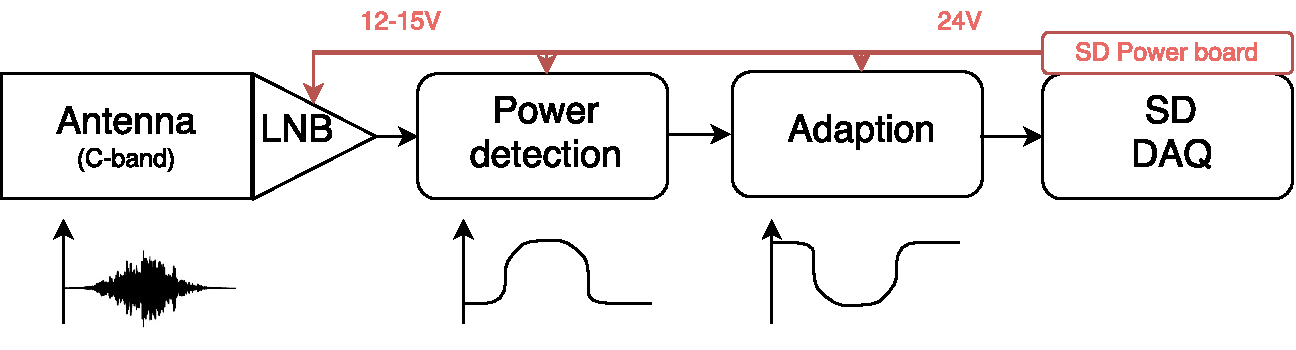
\includegraphics[width=0.69\linewidth]{blockdiagram.pdf}}  
  \caption{block diagram of an EASIER detector unit}
  \label{fig:diagram}  
\end{figure}

\subsubsection*{EASIER61}
A first  array of  seven detectors was  installed at the  Pierre Auger
Observatory  in April  2011.  The  good operation  and results  of this
first test  bed led to an  extension of 54 more  detectors covering a total
instrumented surface  of \unit[91]{$\rm km^2$}.  The  type of antenna used for
this setup  is a  commercial cylindrical horn  antenna with  a maximum
gain of around 9dB, it points to  the zenith and has a half power beam
width (HPBW)  of 90 degrees. The  first seven LNBf are  of the model GI301
made by Global Intersat and  the 54 units of the extension are from
WSInternational, model DMX241. The sensors, composed of the antenna and
the amplification system,  are installed on top of  the SD station (cf
Fig.~\ref{fig:detector} left) and the electronics box is located below
the hatch  box on top  of the SD  electronics.  The EASIER61  array is
located in  the south west part  of the Pierre  Auger Observatory, its
footprint is  shown in Fig.~\ref{fig:detector} (right).   On the total
of  61   antennas,  33  have   a  North-South  polarization,   and  28
East-West.\\ Several radio events in coincidence with an  EAS were measured  with EASIER61 which validated the concept. However, the distance from the antenna to the shower axis of these events are of the order of a few hundreds of meters, thus they can be also attributed to a coherent emission like the ones measured at lower frequency.
\begin{figure}[!ht]
  \centering
  \hspace*{-3ex}  
  \subfigure{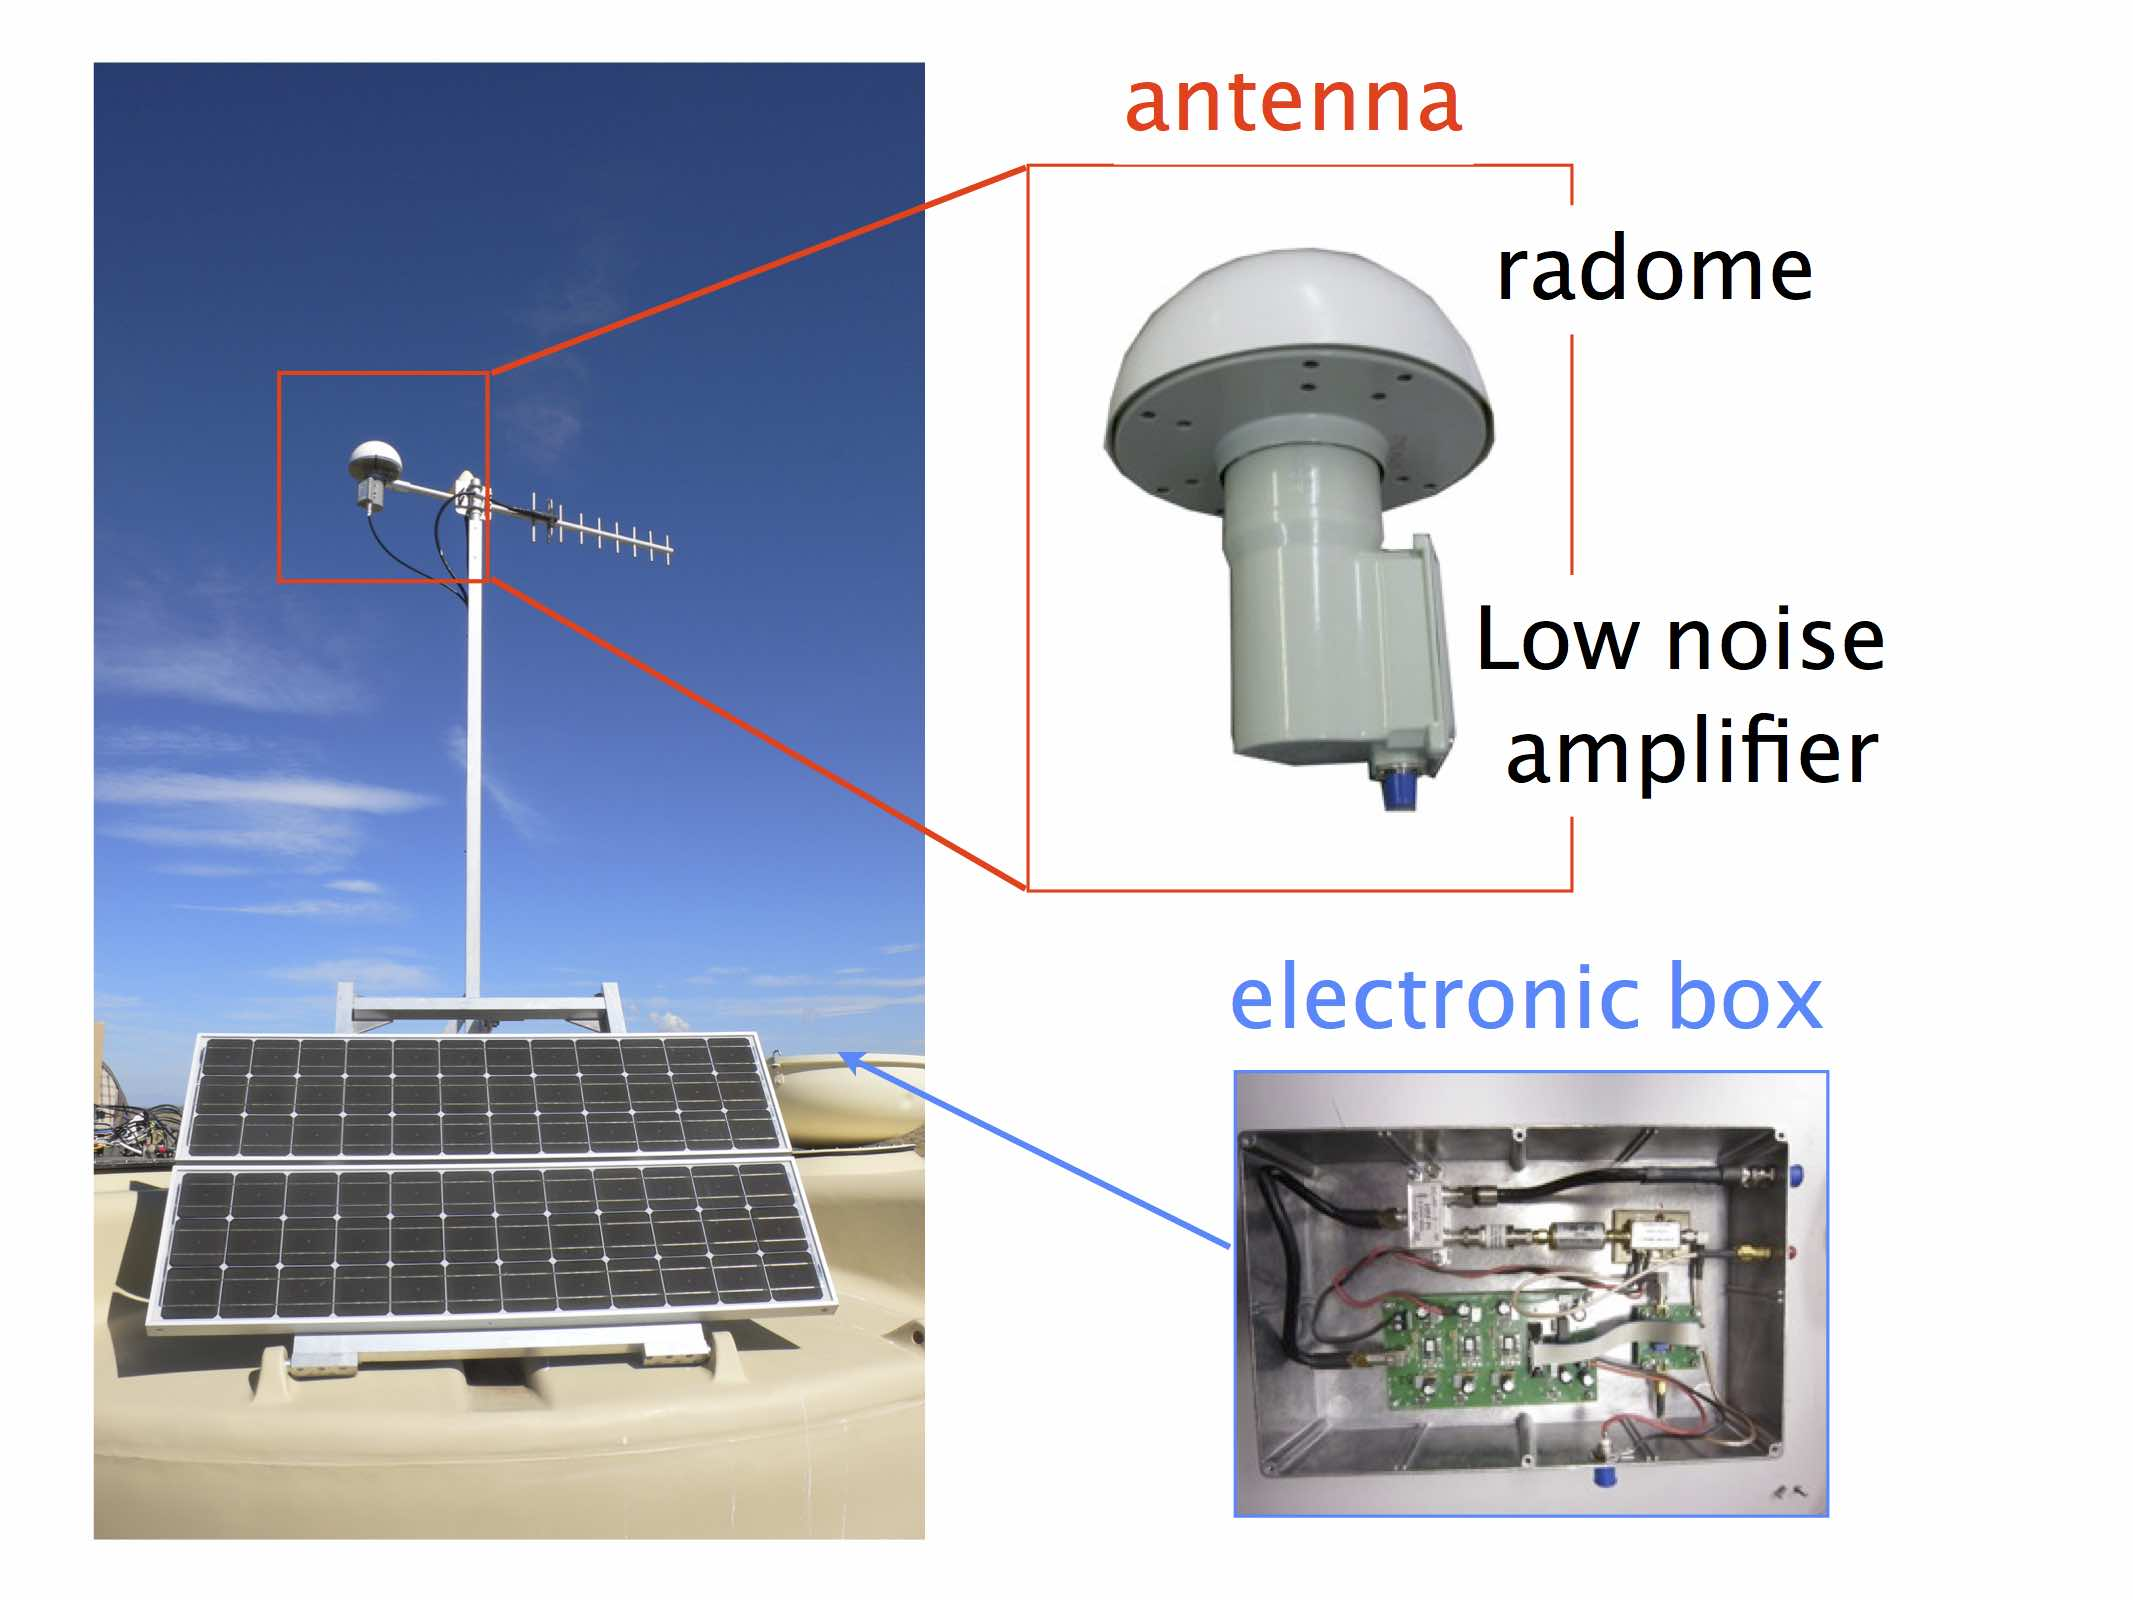
\includegraphics[width=0.49\linewidth]{setupGHznew.jpg}}
  \subfigure{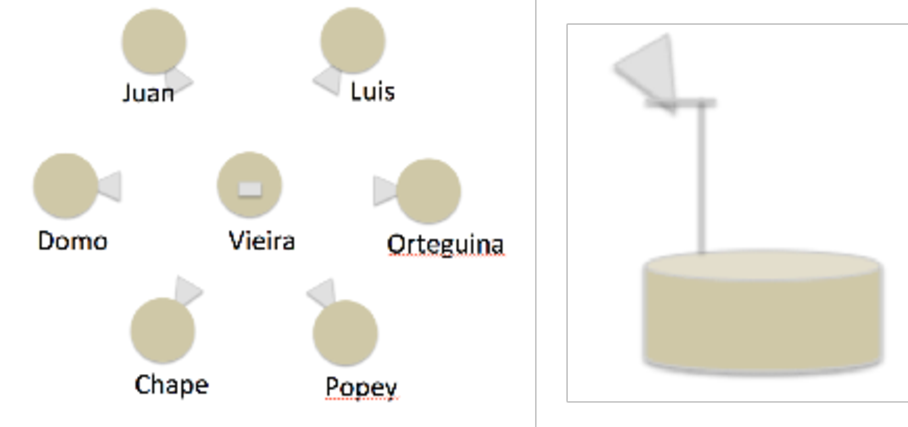
\includegraphics[width=0.49\linewidth]{GD.pdf}}
  \caption{Left: EASIER  detector installed on a  Pierre Auger surface
    detector. Right: Top  view of GIGADuck array  and side view  of one of
    the detector.}
  \label{fig:detector}  
\end{figure}

\subsubsection*{GIGADuck}
A recent calculation  of the MBR signal pointed  out that the expected
signal should  be lower by two orders of  magnitude than the
first estimation presented in~\cite{Gorham}. This consideration led to
the  design  and  the  installation  in March  2015  of  GIGADuck,  an
optimized array  of seven detectors with  a higher gain  antenna and a
different  geometry.   A pyramidal horn of 15dB  gain  antenna from A-Info company increases the  maximum antenna effective area by a factor six with respect to EASIER61.  Furthermore, the array is now composed of a central detector pointing to the zenith and the six peripheral detectors are tilted by 20$\rm ^{\circ} $ in zenith and have their azimuth adjusted to point towards the central detector as represented on the scheme of the Fig.~\ref{fig:GD}.  This configuration  increases the overlap of the detectors' field of view and enhance the probability to obtain a coincident detection. This configuration was chosen because the observation of a coincidence between two radio detectors would support the hypothesis of an isotropic emission.\\
%The  optimized  tilt angle  was  found  as  a compromise  between  the coincidence  probability  and the  antenna  temperature increase  (the brightness temperature  of the sky  increases with the  zenith angle).
As an example of the improved performance of GIGADuck, we show the simulation of the MBR of a vertical 10 EeV shower collected with  an EASIER and a GIGADuck antenna at a distance of  \unit[750]{m}. In this particular case, the ratio between GD and EASIER is around 2 for the vertical and around 10 for the tilted GIGADuck antenna. These differences is the combination of a higher of GIGADuck antenna (illustrated by the vertical antenna comparison) and the part of the shower pointed by the main lobe (illustrated by the large improvement of the inclined case). Further comparison of their performances are given in section~\ref{simulation}.

\begin{figure}[!ht]
  \centering
  \hspace*{-3ex}  
  \subfigure{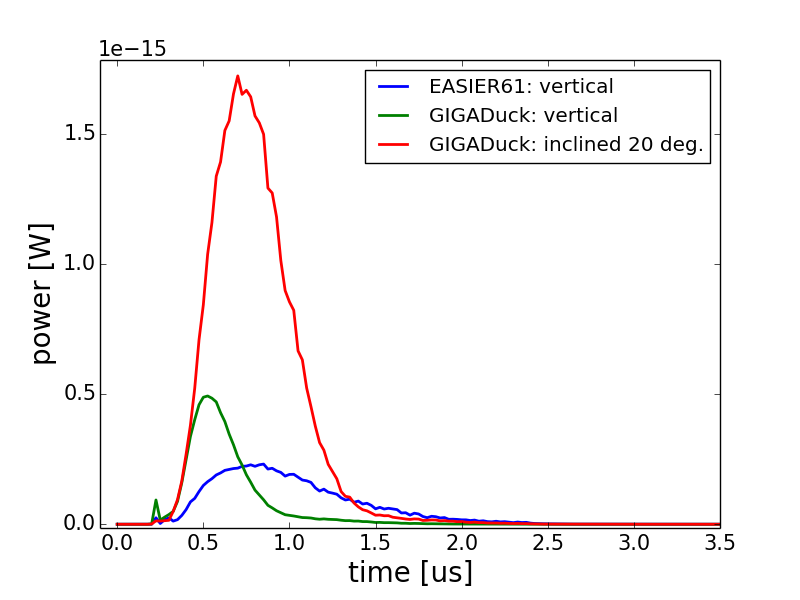
\includegraphics[width=0.49\linewidth]{EAGDexample.png}}
  \caption{Left: Top  view of GIGADuck array  and side view  of one of
    the detector.   Right: Maximum power  received from a  vertical 10
    EeV shower as  a function of its core distance  from an antenna in
    an EASIER-like configuration and a GIGADuck configuration.}
  \label{fig:GD}  
\end{figure}
